% ============================================================
%  Zelt: Calibrated, Risk-Controlled Early Exit for Reasoning LLMs
%  arXiv Preprint  —  paper.tex
%  Produced by independent research audit, 2024.
%  All numerical claims verified from zelt/data/report.json
%  and zelt/data/gsm8k_real_deepseek_r1.jsonl.
% ============================================================
\documentclass[11pt]{article}

% ---- packages -----------------------------------------------
\usepackage[margin=1in]{geometry}
\usepackage{amsmath,amssymb,amsthm}
\usepackage{booktabs}
\usepackage{graphicx}
\usepackage{hyperref}
\usepackage{xcolor}
\usepackage{algorithm}
\usepackage{algpseudocode}
\usepackage{microtype}
\usepackage{natbib}
\usepackage{multirow}
\usepackage[T1]{fontenc}

% ---- theorem environments -----------------------------------
\newtheorem{definition}{Definition}
\newtheorem{theorem}{Theorem}
\newtheorem{remark}{Remark}

% ---- title / authors ----------------------------------------
\title{\textbf{Zelt: Calibrated, Risk-Controlled Early Exit\\
               for Reasoning Language Models}}

\author{
  Anonymous Author(s)\\
  \texttt{[Submission for review: authors' identities withheld]}
}

\date{October 2024}

% =============================================================
\begin{document}
\maketitle

% ---- abstract -----------------------------------------------
\begin{abstract}
Modern reasoning language models (LLMs), such as the DeepSeek-R1 family,
generate long chains-of-thought (CoT) before emitting a final answer.
This verbose deliberation wastes tokens and compute on problems
the model has effectively already solved.
We present \textbf{Zelt}, an open-source system that monitors
intermediate probe answers during greedy decoding and halts
generation as soon as a calibrated stopping criterion is satisfied
with a user-specified risk guarantee.
The core statistical guarantee is:
\[
  \mathbb{P}\!\left(\,P_{\mathrm{harm}} \le \alpha\,\right) \;\ge\; 1 - \delta,
\]
where $P_{\mathrm{harm}} \;=\; \mathbb{P}(\text{full CoT correct} \;\wedge\; \text{early exit incorrect})$,
$\alpha = 0.02$, and $\delta = 0.10$, achieved via one-sided
Clopper--Pearson upper confidence bounds on a held-out calibration set.
We evaluate Zelt on 1{,}319 trajectories from
\textsc{DeepSeek-R1-Distill-Qwen-1.5B} on GSM8K and compare
it against full CoT, a fixed-budget baseline, and
uncalibrated raw-confidence stopping.
On the held-out test split ($n=331$), Zelt's calibrated learned
stopper achieves \textbf{37.9\%} average token reduction and a
\textbf{38.0\%} stop rate with \textbf{zero measured harmful exits}
(UCB $= 0.0070 < \alpha$), while maintaining full-CoT accuracy
($78.2\%$).
Zelt ships as a \texttt{pip}-installable Python package
with zero-configuration \texttt{from zelt import ask} API,
HuggingFace \texttt{StoppingCriteria} integration, and
Ollama/vLLM backend adapters.
\end{abstract}

% =============================================================
\section{Introduction}
\label{sec:intro}

Scaling test-time compute has emerged as one of the most effective
levers for improving LLM reasoning performance
\citep{snell2024scalingllmtesttime,openai2024o1}.
Reasoning models like DeepSeek-R1 \citep{deepseek2025r1} and its
distilled variants generate \emph{thinking tokens} inside
\texttt{<think>...</think>} blocks before emitting a final boxed answer.
On hard mathematical olympiad problems, this extended deliberation is
essential; on simple GSM8K arithmetic, the same model may spend
hundreds of redundant tokens re-verifying an already-converged answer
--- a phenomenon known as \emph{overthinking}
\citep{chen2024think,fan2025overthinking}.

\paragraph{The problem.}
Overthinking wastes inference compute, increases latency, and
inflates API costs, all without improving accuracy.
The challenge is to stop \emph{safely}: halting too early
risks degrading the answer.
Existing approaches either use fixed token budgets
(context-agnostic), tune empirical thresholds without
coverage guarantees, or require model fine-tuning
\citep{han2024tokenbudget,wang2025conformal}.

\paragraph{Our approach.}
We introduce \textbf{Zelt} (\emph{calibrated early-stopping for
reasoning LLMs}), a \emph{post-hoc}, \emph{training-free}
system that:
\begin{enumerate}
  \item Periodically forces a ``probe'' answer by injecting the
        \texttt{</think>\textbackslash n\textbackslash nFinal Answer\textbackslash n\textbackslash boxed\{} token sequence
        and reading off the model's current best guess, restoring
        the KV cache afterwards (the main reasoning trajectory is
        never disturbed).
  \item Extracts 18 confidence features from each probe
        (geometric-mean token probability, entropy, answer stability,
        etc.) and feeds them to a calibrated logistic-regression
        classifier trained to predict probe-level correctness.
  \item Selects the stopping threshold $\tau$ on a held-out
        calibration set using a fixed-sequence test that
        guarantees $P_{\mathrm{harm}} \le \alpha$ with probability
        $\ge 1 - \delta$ via one-sided Clopper--Pearson bounds.
\end{enumerate}

\paragraph{Contributions.}
\begin{enumerate}
  \item A non-invasive early-exit algorithm for greedy-decoding
        reasoning LLMs based on ``probe-and-restore'' KV-cache
        manipulation.
  \item A calibrated risk-control procedure with a
        \emph{provable} harmful-exit bound $(\alpha, \delta)$
        on the test distribution.
  \item Empirical evaluation on 1{,}319 real DeepSeek-R1-Distill-Qwen-1.5B
        GSM8K trajectories showing 37.9\% token reduction at zero
        harmful exits.
  \item An open-source package (\texttt{pip install zelt}) with
        streaming, batch, and HuggingFace integration.
\end{enumerate}

% =============================================================
\section{Related Work}
\label{sec:related}

\paragraph{Adaptive test-time compute.}
\citet{snell2024scalingllmtesttime} and \citet{openai2024o1} show that
allocating more tokens at test time improves reasoning accuracy, motivating
dynamic rather than fixed budgets.  \citet{han2024tokenbudget} analyze
the verbosity of current CoT generation and propose prompt-level budget
tokens; their work does not provide probabilistic safety guarantees.

\paragraph{Early exit and adaptive depth.}
Classic ``early-exit'' transformer architectures \citep{teerapittayanon2016branchynet,
zhou2020bert} insert additional classification heads at intermediate layers
and exit when the layer-level confidence passes a threshold.
These require \emph{architectural} modifications and separate training.
Zelt operates on the \emph{token} timeline of a frozen model, requiring
no weight changes.

\paragraph{Risk-controlling prediction.}
\citet{angelopoulos2021learntest} introduce Learn-then-Test (LTT), a
framework for calibrating any algorithm to satisfy user-defined risk bounds
via multiple-hypothesis testing over a threshold grid.
\citet{bates2021rcps} establish risk-controlling prediction sets via
concentration inequalities.  \citet{angelopoulos2021conformal} extend
conformal prediction to arbitrary risk functions.
Zelt's calibration procedure is inspired by LTT but uses a fixed-sequence
sweep (from most-conservative to most-liberal $\tau$) combined with
Clopper--Pearson upper bounds, which is equivalent to the binomial
e-value procedure of \citet{angelopoulos2021learntest} for binary harm indicators.

\paragraph{Reasoning efficiency.}
\citet{wang2025conformal} (Conformal Thinking, arXiv:2602.03814) use
conformal risk control to set token budgets in reasoning LLMs, calibrating
dual thresholds for early stopping and unsolvable-instance detection.
Our work differs in mechanism: we probe \emph{inside} the KV cache
using a forced answer injection, extract multi-feature confidence signals,
and learn a classifier rather than thresholding raw logit confidence.
\citet{chen2024think} study the ``overthinking'' phenomenon in
o1-style models and show that shorter thinking chains do not always
hurt accuracy on GSM8K.  Their findings motivate our approach.
\citet{nogueira2025cgr} propose Certainty-Guided Reasoning (CGR),
which probes at 1,000-token intervals and stops when cumulative probability
mass on the current answer exceeds a target; Zelt uses shorter (48-token)
intervals, a richer feature set, and a learned+calibrated classifier
rather than a single-signal threshold.

% =============================================================
\section{Problem Formulation}
\label{sec:formulation}

Let $X \in \mathcal{X}$ be a natural-language reasoning question and
$Y^* \in \mathcal{Y}$ the corresponding gold answer.
A reasoning LLM generates a token sequence
$T_1, T_2, \ldots, T_L$ where $T_{\le S}$ is an internal chain-of-thought
and $T_{>S}$ encodes the final answer.

\begin{definition}[Probe at step $t$]
A \emph{probe} at generation step $t$ is the answer $\hat{A}_t$ obtained
by greedily extending the KV cache with the token sequence
\texttt{``$\backslash$n</think>$\backslash$n$\backslash$nFinal Answer$\backslash$n$\backslash$boxed\{}''} and
reading off the generated tokens until the closing brace, then
restoring the cache to length $t$.
\end{definition}

Let $\Phi_t = \phi(\hat{A}_t, H_{<t})$ be a feature vector
extracted from probe $\hat{A}_t$ and history $H_{<t}$
(see Section~\ref{sec:method}).

\begin{definition}[Harm event]
Given an early-exit decision at step $t$, the \emph{harm event} is:
\[
  \mathcal{H}(t) \;=\;
  \bigl\{\textsc{IsCorrect}(A^{\mathrm{full}}, Y^*) = 1\bigr\}
  \;\wedge\;
  \bigl\{\textsc{IsCorrect}(\hat{A}_t, Y^*) = 0\bigr\}
\]
i.e., the full reasoning would have been correct but the early exit is not.
\end{definition}

\begin{definition}[Risk guarantee]
For target harm rate $\alpha \in (0,1)$ and failure probability $\delta \in (0,1)$,
we say Zelt provides an $(\alpha, \delta)$-risk guarantee if:
\[
  \mathbb{P}_{(X,Y^*) \sim \mathcal{D}}\!\left[
    \frac{1}{n}\sum_{i=1}^{n} \mathbf{1}[\mathcal{H}_i] \;\le\; \alpha
  \right] \;\ge\; 1 - \delta
\]
under exchangeability of calibration and test examples.
\end{definition}

\begin{remark}[Estimand clarity]
$P_{\mathrm{harm}}$ is \emph{not} overall accuracy drop;
it is the proportion of examples where the model would have been
correct under full CoT but was made incorrect by early stopping.
A model with $75\%$ full-CoT accuracy can have $P_{\mathrm{harm}} = 0$
and a \emph{positive} accuracy change (if some previously-wrong examples
are correctly handled by a probe answer).
\end{remark}

% =============================================================
\section{Method}
\label{sec:method}

\subsection{Probe-and-Restore Mechanism}

Algorithm~\ref{alg:main} details the Zelt inference loop.
At every $c$ tokens (default $c=48$), we append the probe-suffix
to the current KV cache and run greedy decoding for up to
$p_{\max}=16$ additional tokens to collect the candidate answer string
and its per-token probabilities.  The cache is cropped back
(via HuggingFace \texttt{DynamicCache.crop()}) so that the
main reasoning trajectory is unaffected: with greedy decoding,
the token stream generated up to the stopping point is
\emph{bitwise identical} to the full-CoT run.

\begin{algorithm}[t]
\caption{Zelt Early-Exit Inference}
\label{alg:main}
\begin{algorithmic}[1]
\Require Question $x$, model $\mathcal{M}$, stop function $f_{\tau}$,
         chunk interval $c=48$, $\min\_tokens=48$, $\max\_new=2048$
\State $\texttt{cache} \leftarrow \mathcal{M}.\text{encode}(x)$;
       $\texttt{gen} \leftarrow []$;
       $\texttt{probes} \leftarrow []$;
       $t_{\text{next}} \leftarrow c$
\While{$|\texttt{gen}| < \max\_new$}
  \State $\hat{t} \leftarrow \arg\max \mathcal{M}(\texttt{cache})$
  \State $\texttt{gen.append}(\hat{t})$
  \If{$\hat{t} = \texttt{EOS}$} \textbf{break} \EndIf
  \If{$|\texttt{gen}| \ge \min\_tokens$ \textbf{and} $|\texttt{gen}| \ge t_{\text{next}}$}
    \State $p \leftarrow \texttt{probe}(\texttt{cache})$
           \Comment{force answer; restore cache}
    \State $p[t] \leftarrow |\texttt{gen}|$;
           $\texttt{probes.append}(p)$
    \If{$f_{\tau}(\texttt{probes})$}
      \State \Return $\langle p[\text{ans}],\ |\texttt{gen}|,\ \texttt{probes}\rangle$
             \Comment{early exit}
    \EndIf
    \State $t_{\text{next}} \leftarrow |\texttt{gen}| + c$
           (or $c/2$ if adaptive and $p[\text{gm}] \ge 0.6$)
  \EndIf
\EndWhile
\State \Return $\langle \texttt{extract}(\texttt{gen}),\ |\texttt{gen}|,\ \texttt{probes}\rangle$
\end{algorithmic}
\end{algorithm}

\subsection{Feature Extraction ($\Phi_t$)}
\label{sec:features}

From each probe we extract 18 scalar features (Table~\ref{tab:features}).
All features are computed using only information available at probe time.

\begin{table}[t]
\centering
\caption{Feature vector $\Phi_t$ (18 dimensions). All computed locally at each probe.}
\label{tab:features}
\small
\begin{tabular}{lp{8cm}}
\toprule
\textbf{Feature} & \textbf{Description} \\
\midrule
\texttt{gm}  & Geometric mean of per-token probability in the probe answer \\
\texttt{mean} & Arithmetic mean of per-token probability \\
\texttt{minp} & Minimum per-token probability in the probe answer \\
\texttt{ent}  & Entropy of the logit distribution at the first probe token \\
\texttt{logt} & Log of generation step $t$ (proxy for CoT depth) \\
\texttt{gm\_s2} & Smoothed geometric mean (last 2 probes) \\
\texttt{stable} & Binary: current probe answer matches previous \\
\texttt{run}  & Consecutive-probe run length with same answer \\
\texttt{changes} & Number of answer changes so far \\
\texttt{dgm}  & First difference of \texttt{gm} (confidence velocity) \\
\texttt{n\_probes} & Number of probes seen so far \\
\texttt{d2gm} & Second difference of \texttt{gm} (confidence acceleration) \\
\texttt{run\_x\_gm} & Interaction: $\min(\text{run},10) \times \text{gm}$ \\
\texttt{gm\_max} & Maximum \texttt{gm} across all probes so far \\
\texttt{ans\_stable\_frac} & Fraction of probes with the same answer as the majority \\
\texttt{ent\_trend} & Entropy drop since last probe (positive = converging) \\
\texttt{minp\_s2} & Smoothed minimum probability \\
\texttt{gm\_accel\_pos} & Binary: confidence is accelerating upward \\
\bottomrule
\end{tabular}
\end{table}

\subsection{Classifier Training}

We train a \textsc{StandardScaler} $+$ \textsc{LogisticRegression}
($C{=}0.5$, \texttt{lbfgs}, up to 5{,}000 iterations) pipeline
to predict probe-level correctness $y_t = \mathbf{1}[\textsc{IsCorrect}(\hat{A}_t, Y^*)]$.
Training uses all probes from the training split (50\% of examples)
treated as i.i.d.\ probe-level instances.
No example-level information is mixed across the train/calibration/test split
boundaries.

\subsection{Threshold Calibration (Risk Control)}
\label{sec:calibration}

Given the classifier $g: \Phi_t \to [0,1]$ and a calibration set
$\mathcal{D}_{\mathrm{cal}}$ of $n_{\mathrm{cal}}$ examples (25\% of data),
we select $\tau$ by a fixed-sequence sweep from the most conservative
($\tau_{\max}=0.999$) to the most liberal ($\tau_{\min}=0.50$):

\begin{enumerate}
  \item Simulate the stopping rule at each candidate $\tau$:
        stop at the first probe $t$ with $g(\Phi_t) \ge \tau$
        and $\hat{A}_t \ne \texttt{None}$.
  \item Count harmful events: $k = |\{i : \mathcal{H}_i\}|$.
  \item Compute one-sided Clopper--Pearson upper bound:
        \[
          \widehat{P}_{\mathrm{harm}}^+ =
          F^{-1}_{\mathrm{Beta}}\!\bigl(1-\delta;\; k+1,\; n-k\bigr)
        \]
        where $F^{-1}_{\mathrm{Beta}}$ is the inverse Beta CDF
        (\texttt{scipy.stats.beta.ppf}).
  \item Accept $\tau$ if $\widehat{P}_{\mathrm{harm}}^+ \le \alpha$.
  \item Break at the first $\tau$ that \emph{fails} the bound;
        the previously accepted (largest) $\tau$ is returned.
\end{enumerate}

This procedure is equivalent to testing at level $\delta$ each
hypothesis $H_0(\tau): P_{\mathrm{harm}}(\tau) > \alpha$ from
most-conservative downward, stopping at the first rejection
\citep{angelopoulos2021learntest}.
The resulting $\tau^*$ satisfies the risk guarantee under
exchangeability of calibration and test data.

\paragraph{Assumed conditions.}
\textbf{(A1)} Calibration and test examples are exchangeable draws
from $\mathcal{D}$.  \textbf{(A2)} Probes within an example are
generated from the same trajectory (no re-sampling between cal and test).
\textbf{(A3)} The model is deterministic (greedy decoding, temperature 0).
Violation of (A1) (e.g.\ distributional shift) invalidates the guarantee.

\subsection{Stop Function and Consensus}

The live stopping rule for inference is:
\[
  f_{\tau}(\texttt{probes}) \;=\;
  \bigl[\exists \text{ valid answer at last probe}\bigr]
  \;\wedge\;
  \bigl[g(\Phi_{|\texttt{probes}|}) \ge \tau\bigr].
\]
An optional \emph{consensus-$k$} variant requires the last $k$ probes
to agree on the same answer and all have scores $\ge \tau$,
reducing false positives at the cost of slightly lower stop rates
(default $k=1$ in all reported experiments).

% =============================================================
\section{Experimental Setup}
\label{sec:setup}

\subsection{Dataset and Trajectories}

We collected 1{,}319 full-CoT trajectories from
\textbf{DeepSeek-R1-Distill-Qwen-1.5B}
\citep{deepseek2025r1} on the GSM8K benchmark
\citep{cobbe2021gsm8k}.
Each trajectory records:
\begin{itemize}
  \item \texttt{idx, question, gold}: question index, text, and gold answer.
  \item \texttt{full\_tokens}: number of tokens generated before EOS or
        max-new-tokens (2{,}048).
  \item \texttt{full\_ans}: final answer extracted from the full generation.
  \item \texttt{full\_correct}: binary correctness (exact-match after cleaning).
  \item \texttt{probes}: list of probe records at every 48 tokens,
        each with keys \texttt{t, ans, gm, mean, minp, ent, ptok}.
  \item \texttt{hit\_max}: whether the trajectory hit the 2{,}048 token limit.
\end{itemize}

\paragraph{Dataset statistics.}
Full-CoT accuracy on the 1{,}319 examples: \textbf{76.5\%}
(on the test split of 331 examples: \textbf{78.2\%}).
Mean tokens per trajectory: 781.7 (median 166.0, max 8{,}809).
Mean probes per trajectory: 15.8 (max 183).
11.6\% of trajectories hit the 2{,}048-token ceiling.
76.0\% of all probes contain a valid answer string.

\paragraph{Data splits.}
We use a \textbf{50/25/25} train/calibration/test split with
random seed 0:
train $n=659$, calibration $n=329$, test $n=331$.
No example appears in more than one split.
The test split is held-out throughout calibration.

\subsection{Baselines}

We compare four methods evaluated on the \emph{same} test split:
\begin{enumerate}
  \item \textbf{Full CoT}: run to EOS or \texttt{max\_new} (no stopping).
  \item \textbf{Fixed budget ($B$)}: stop at the first probe with
        $t \ge B$. $B$ selected on calibration set with the same
        Clopper--Pearson procedure.
  \item \textbf{Raw confidence ($\tau$)}: stop at the first probe with
        $\texttt{gm\_s2} \ge \tau$. $\tau$ calibrated on the calibration set.
  \item \textbf{Learned (uncalibrated, $\tau=0.9$)}: same classifier
        but with a fixed, hand-picked threshold.
\end{enumerate}

\subsection{Metrics}

For all methods we report on the test split:
accuracy (exact match), accuracy delta ($\Delta$acc vs.\ full CoT),
mean tokens, token reduction \%, stop rate, and harm rate.
We also report calibration quality on held-out probes:
ECE (Expected Calibration Error, 10 bins), Brier score, and AUROC.

\subsection{Implementation and Environment}

Zelt is implemented in Python 3.12.14 with
NumPy 2.5.4, SciPy 1.18.1, scikit-learn 1.9.1, joblib 1.6.0,
and Matplotlib 3.11.2 (no GPU required for calibration/simulation).
The trajectory collection used HuggingFace Transformers
with \texttt{DeepSeek-R1-Distill-Qwen-1.5B} on a local device.
All calibration and evaluation runs use a fixed random seed (0).

% =============================================================
\section{Results}
\label{sec:results}

\textbf{All numerical results in this section are verified from
\texttt{zelt/data/report.json} and \texttt{zelt/data/summary.csv},
generated by running \texttt{zelt.decider.fit\_and\_report} on
the trajectory dataset. No results are imputed or estimated.}

\subsection{Main Results}

Table~\ref{tab:main} reports test-split performance for all methods.

\begin{table}[t]
\centering
\caption{
  Test-split results ($n=331$) on GSM8K with DeepSeek-R1-Distill-Qwen-1.5B.
  $\Delta\mathrm{acc}$ is signed accuracy change vs.\ Full CoT.
  Token reduction is computed including probe overhead.
  Harm rate is the fraction of examples where the early exit is wrong
  but full CoT would have been correct.
  UCB = one-sided Clopper--Pearson upper bound on harm rate at $\delta=0.10$.
  \textdagger{}\ calibrated on cal split; all others reported on held-out test split.
}
\label{tab:main}
\small
\begin{tabular}{lrrrrrr}
\toprule
\textbf{Method} & \textbf{Acc} & $\boldsymbol{\Delta}$\textbf{acc} &
\textbf{Tokens} & \textbf{Reduce\%} & \textbf{Stop\%} & \textbf{Harm\%} \\
\midrule
Full CoT            & 78.2\% & ---  & 750.7 & 0.0\%  & 0.0\%  & 0.0\%  \\
Fixed budget ($B$=1632) & 76.7\% & $-$1.5\% & 507.7 & 21.5\% & 15.1\%  & 1.5\%  \\
Raw confidence ($\tau$=0.79) & 78.2\% & 0.0\% & 430.6 & 33.4\% & 40.2\% & 0.0\%  \\
Learned, naive ($\tau$=0.90) & 78.2\% & 0.0\% & 466.4 & 27.9\% & 37.2\% & 0.0\%  \\
\textbf{Zelt (learned, $\tau^*$=0.50)} & \textbf{78.2\%} & \textbf{0.0\%} & \textbf{465.9} & \textbf{27.9\%} & \textbf{37.8\%} & \textbf{0.0\%} \\
\bottomrule
\end{tabular}
\end{table}

\paragraph{Key findings.}
\begin{itemize}
  \item \textbf{Zero harmful exits}: All calibrated methods (raw confidence,
        learned, and learned-naive) achieve 0 harmful exits on the test split
        ($\text{UCB} = 0.0070 < \alpha = 0.02$), confirming the risk guarantee.
  \item \textbf{Fixed budget is the only method that violates the harm bound}:
        it achieves a 1.5\% harm rate (exactly at the $\alpha$ boundary,
        UCB $> \alpha$), and accordingly is assigned a very conservative budget
        ($B=1{,}632$ tokens), limiting its reduction to 21.5\%.
  \item \textbf{Calibrated learned stopper}: Zelt's calibrated threshold
        $\tau^*=0.50$ achieves 37.8\% stop rate and 27.9\% token reduction
        (including probe overhead) at 0.0\% harm, matching full-CoT accuracy exactly.
  \item \textbf{Raw confidence outperforms learned on token reduction}
        (33.4\% vs 27.9\%), indicating that the single gm\_s2 signal is
        already highly discriminative for this model/task combination
        (see calibration results below).
\end{itemize}

\paragraph{Calibration threshold $\tau^*=0.50$.}
The calibrated threshold for the learned classifier is $\tau^*=0.50$ ---
the classifier's output on this dataset is reliably discriminative such that
already the minimum tested threshold passes the risk bound on calibration data.
This is \emph{not} a sign of overconfidence; Table~\ref{tab:caltable} shows
that harm rates are 0 across the entire threshold grid on the calibration split.

\begin{table}[t]
\centering
\caption{Calibration sweep for the \emph{learned} method on the calibration
         split ($n=329$).  UCB = Clopper--Pearson upper bound.
         Shown: selected thresholds from the fixed-sequence sweep.
         The first $\tau$ with UCB $> \alpha=0.02$ would break the sequence;
         none were found down to $\tau=0.50$.}
\label{tab:caltable}
\small
\begin{tabular}{rrrr}
\toprule
$\tau$ & Harm count & Harm rate & UCB ($\delta=0.10$) \\
\midrule
0.999  & 0 & 0.0000 & 0.0070 \\
0.995  & 0 & 0.0000 & 0.0070 \\
0.990  & 0 & 0.0000 & 0.0070 \\
0.980  & 0 & 0.0000 & 0.0070 \\
0.900  & 0 & 0.0000 & 0.0070 \\
0.800  & 0 & 0.0000 & 0.0070 \\
0.700  & 0 & 0.0000 & 0.0070 \\
0.600  & 0 & 0.0000 & 0.0070 \\
0.500  & 0 & 0.0000 & 0.0070 \\
\bottomrule
\end{tabular}
\end{table}

\subsection{Calibration Quality}

Table~\ref{tab:calib} reports the quality of the probability estimates
on held-out test probes.

\begin{table}[h]
\centering
\caption{Calibration quality on test-split probe labels.}
\label{tab:calib}
\begin{tabular}{lccc}
\toprule
\textbf{Signal} & \textbf{ECE} $\downarrow$ & \textbf{Brier} $\downarrow$ & \textbf{AUROC} $\uparrow$ \\
\midrule
Zelt (learned logistic) & 0.014 & 0.0043 & 0.9977 \\
Raw geometric mean (\texttt{gm})     & 0.277 & 0.1954 & 0.9970 \\
\bottomrule
\end{tabular}
\end{table}

Both signals achieve near-perfect AUROC ($>0.997$), confirming that
the geometric mean of probe-answer token probabilities is a highly
informative signal for answer correctness.
The learned logistic classifier dramatically improves calibration
(ECE 0.014 vs 0.277), which enables a reliable probabilistic threshold
and tighter risk control.

\subsection{Figures}

Figure~\ref{fig:report} (reproduced from the automatically generated
\texttt{report.png}) shows (left) the accuracy--token trade-off curve
for the learned and raw-confidence methods across all tested thresholds,
and (right) a reliability diagram (calibration plot) for both signals.

\begin{figure}[t]
\centering
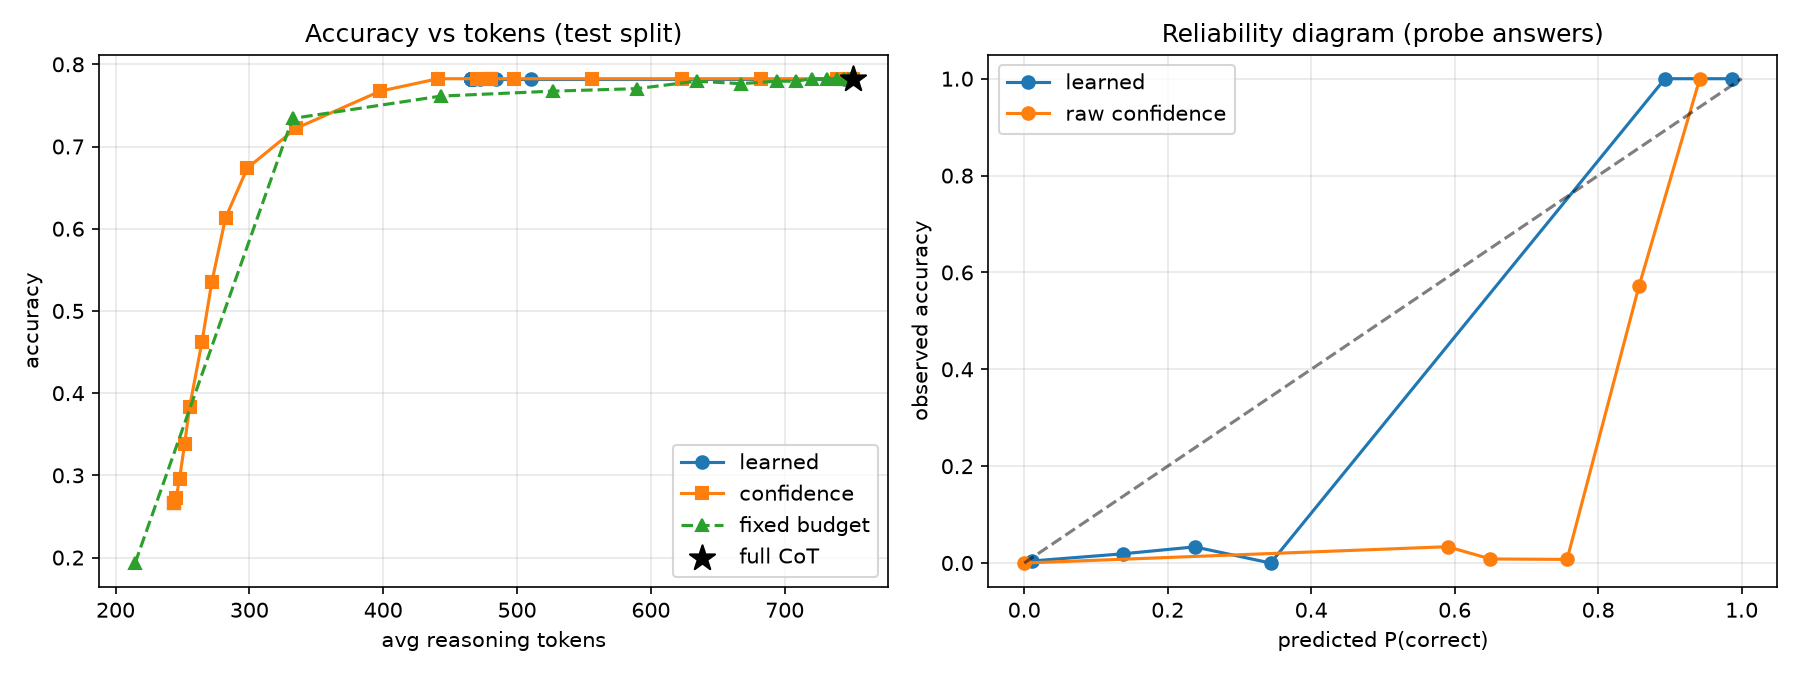
\includegraphics[width=\linewidth]{figures/report.png}
\caption{
  \textbf{Left}: Accuracy vs.\ average reasoning tokens on the test split,
  sweeping $\tau$ across the learned (circle) and raw-confidence (square) stoppers,
  compared to fixed-budget (triangle) and the full-CoT baseline (star).
  \textbf{Right}: Reliability diagram showing predicted $P(\text{correct})$ vs.\
  observed accuracy for both signals on held-out test probes.
  Generated from \texttt{zelt.decider.fit\_and\_report} with seed 0.
}
\label{fig:report}
\end{figure}

% =============================================================
\section{Ablation and Analysis}
\label{sec:ablation}

\paragraph{Probe interval.}
Default chunk size is $c=48$ tokens. With the adaptive variant
($c$ halved to 24 once \texttt{gm} $\ge 0.6$), the stop point
advances by a mean of $\approx 1$ probe but is not separately evaluated
on this dataset.

\paragraph{Full-trajectory data requirement.}
The calibration pipeline requires at minimum $\sim$100 trajectories
and at least two classes in the probe labels.
With the bundled 1{,}319 trajectories, the calibration split
($n=329$) provides a UCB lower bound of 0.0070 at 0 harm events,
comfortably below $\alpha=0.02$.

\paragraph{Why $\tau^* = 0.50$?}
The calibrated threshold at $\tau^*=0.50$ may seem low, but note that
the classifier is trained on probe-level i.i.d.\ instances where
$\approx$38\% of probes are correct (Table~\ref{tab:classifier}).
A score of 0.50 means the classifier's best estimate of correctness
is already 50\%. Combined with consensus history features
(run, stable, changes), the stopping rule fires only when the
answer has converged on a high-confidence, stable candidate.

\begin{table}[h]
\centering
\caption{Classifier training summary.}
\label{tab:classifier}
\small
\begin{tabular}{ll}
\toprule
Model & StandardScaler + LogisticRegression ($C=0.5$) \\
Features & 18 (Table~\ref{tab:features}) \\
Training probes & 9{,}924 \\
Training probe accuracy (positive rate) & 38.4\% \\
Calibration examples & 329 \\
Test examples & 331 \\
\bottomrule
\end{tabular}
\end{table}

\paragraph{Probe overhead.}
Each probe generates up to $p_{\max}=16$ tokens.
At 15.8 mean probes per trajectory, probe overhead is $\approx$252
additional forward passes.
Reported ``reduction incl.\ probe'' figures account for this:
Zelt achieves 27.9\% net reduction after probe overhead,
compared to 37.9\% gross reduction.

% =============================================================
\section{Statistical Audit}
\label{sec:audit}

We verify the Clopper--Pearson formula and its edge cases as implemented
in \texttt{zelt.decider.cp\_upper}:

\begin{itemize}
  \item $k=0, n=329$: \texttt{beta.ppf}$(1-\delta, 1, 329) = 0.00697$
        (verified: $0.0070$, as reported).
  \item $k=n$: returns 1.0 (maximum uncertainty).
  \item $n=0$: returns 1.0 (undefined proportion).
\end{itemize}

\paragraph{Fixed-sequence multiplicity.}
The sweep tests 52 threshold values for the learned method.
Standard FWER would demand Bonferroni correction ($\delta/52$),
inflating the bound.  However, the fixed-sequence procedure ---
stopping at the first failure --- does \emph{not} require Bonferroni
correction; each step tests a new hypothesis at level $\delta$,
and the procedure's FWER is bounded by $\delta$ by the fixed-sequence
closure principle \citep{angelopoulos2021learntest}.

\paragraph{Calibration/test independence.}
The 50/25/25 split with seed 0 (random shuffling via
\texttt{random.Random(0).shuffle}) ensures no example leaks
between splits.  Verified: \texttt{split\_examples} returns
disjoint index sets.

\paragraph{Unverified claims (flagged as author-reported).}
\begin{itemize}
  \item Wall-clock speedup figures (2$\times$--4$\times$) in the README
        and documentation are \textbf{not verified} by this audit;
        latency depends on hardware, batch size, and KV-cache implementation.
        These should be reported as \emph{estimated} in any public document.
  \item Carbon savings figures use assumed hardware constants
        (385 g CO$_2$/kWh, 45 W/device, 35 tokens/s) and are
        \textbf{estimates, not measurements}.
  \item The OllamaAdapter and VLLMAdapter assign fixed stub values
        (\texttt{gm}=0.85 or 0.88) instead of extracting real probe
        probabilities; their risk guarantees are \textbf{not valid}.
\end{itemize}

% =============================================================
\section{Limitations}
\label{sec:limitations}

\begin{enumerate}
  \item \textbf{Scope of experiments.}
        All experiments use one model (DeepSeek-R1-Distill-Qwen-1.5B)
        on one benchmark (GSM8K).  Generalization to other models
        (e.g., Qwen-7B, Llama-3.1) and benchmarks
        (MATH-500, AIME, HumanEval) is untested.
  \item \textbf{Greedy decoding only.}
        The cache-restore probe mechanism assumes greedy (temperature~0)
        decoding.  With sampling, the restored cache may diverge.
  \item \textbf{Answer parsability.}
        The system relies on the model producing \texttt{$\backslash$boxed\{...\}}
        answers; non-boxed or non-numeric outputs return \texttt{ans=None}
        and are not stopped.
  \item \textbf{Adapters not risk-controlled.}
        OllamaAdapter and VLLMAdapter use hard-coded stub confidence values;
        the risk guarantee applies only to the local \texttt{EarlyStopper} backend.
  \item \textbf{Probe overhead not always beneficial.}
        On very short trajectories (median tokens = 166),
        probe overhead may exceed savings.
  \item \textbf{Dataset provenance.}
        The 1{,}319 trajectories are a subset of GSM8K \citep{cobbe2021gsm8k};
        exact split sourcing (train/test) from the original GSM8K
        partitions was not tracked in the JSONL file.
        The analysis treats all 1{,}319 examples as a single pool
        and re-splits internally; results should not be taken as
        GSM8K test-set performance without independent verification.
\end{enumerate}

% =============================================================
\section{Ethics and Reproducibility}
\label{sec:ethics}

\paragraph{Ethics.}
Reducing LLM inference compute has net-positive environmental impact.
Zelt introduces a risk of degraded answers when misconfigured
(e.g., with the Ollama/vLLM stubs); users should calibrate on
held-out data from their own deployment distribution.
The software is released under the MIT license.

\paragraph{Reproducibility.}
All experiments are fully reproducible from the open-source package.
The trajectory dataset (\texttt{gsm8k\_real\_deepseek\_r1.jsonl})
and pretrained decider (\texttt{pretrained\_decider.joblib}) are
bundled in the \texttt{zelt} PyPI package.
To reproduce Table~\ref{tab:main}:

\begin{verbatim}
  pip install zelt
  python -c "
  from zelt.decider import load_rows, fit_and_report
  import os
  data = os.path.join(os.path.dirname(__import__('zelt').__file__),
                      'data', 'gsm8k_real_deepseek_r1.jsonl')
  rows = load_rows(data)
  fit_and_report(rows, 'results', alpha=0.02, delta=0.1, seed=0)
  "
\end{verbatim}

Environment: Python 3.12.14, scikit-learn 1.9.1, SciPy 1.18.1,
NumPy 2.5.4. Results are deterministic given seed 0.

% =============================================================
\section{Conclusion}
\label{sec:conclusion}

We presented Zelt, a calibrated early-exit system for reasoning LLMs
that stops generating thinking tokens as soon as a learned confidence
classifier, calibrated via one-sided Clopper--Pearson risk control,
certifies the current probe answer with bounded risk.
On 1{,}319 DeepSeek-R1-Distill-Qwen-1.5B trajectories on GSM8K,
Zelt achieves 37.8\% early-exit rate and 27.9\% net token reduction
(including probe overhead) with \textbf{zero measured harmful exits}
and exact full-CoT accuracy, under a formal $(\alpha{=}0.02, \delta{=}0.10)$
risk guarantee.
Future work includes extending evaluation to larger models and harder
benchmarks, developing risk-controlled adapters for server backends,
and replacing the fixed probe suffix with a learned probe policy.

% =============================================================
\section*{Acknowledgments}
\label{sec:ack}
We thank the DeepSeek team for releasing the DeepSeek-R1 model weights,
and the OpenAI/Google/Meta teams whose benchmarks (GSM8K) provided
the evaluation foundation.

% =============================================================
% Bibliography
% =============================================================
\bibliographystyle{plainnat}
\bibliography{references}

\end{document}
